\section{Introduction}
This document outlines the purpose and key components of the Rubin Pixel Zone, which is designed to provide an isolated and secure environment, separate from the broader observatory network and its associated products. The Pixel Zone will house data generated by the LSST camera throughout the duration of the survey. All data classified as “pixel data” must adhere to DOE and NSF access control and security policies.

The term Pixel Zone refers to this isolated network environment, which operates under a distinct routing instance, separate from the Rubin default routing domain. Specifically, it utilizes its own routing table via VRF. 

\section{Network Design}

The following is a high-level design of how the Pixel Zone looks and how it works:

\begin{figure}
    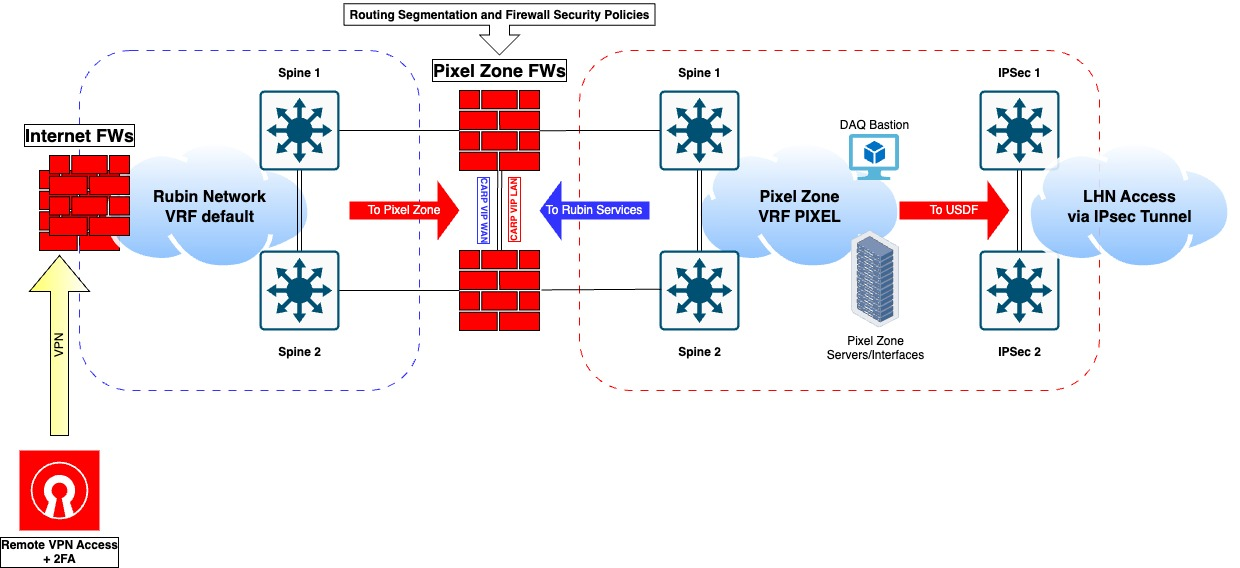
\includegraphics[width=13cm]{pixel_zone.jpg}
    \centering
    \caption*{Logical Topology of Pixel Zone}
\end{figure}

On the left side of the diagram, the default VRF routing is where all the non-Pixel services live. The VRF-PIXEL operates as a completely isolated routing domain. This separation ensures all the components and subsystems interacting with pixel data are logically and securely segmented from the rest of the observatory network. The use of a dedicated VRF enhances both security and compliance by limiting access and enforcing strict boundaries around sensitive data flows.

Spine 1 and Spine 2 refer to the same physical devices located on both sides of the firewall; however, they are configured in two separate VRFs

The IPSec switches provide an encrypted channel to USDF. 

Details of the technical implementation can be reviewed in \href{https://rubinobs.atlassian.net/wiki/x/NAB6IQ}{"Rubin Pixel Zone"}

\section{Subsystems Inside the Pixel Zone}

The following subsystems are inside the pixel zone

\begin{itemize}
    \item Kubernetes Computing cluster
    \item Kubernetes Storage cluster
    \item LSST camera and all its hosts
    \item Control Room Workstations
\end{itemize}

Any other system not in the Pixel Zone that needs to consume its services, it must be authorized in the firewall. 

\section{Consuming Services of the Pixel Zone}

A set of network security rules are  established to ensure the logical isolation of the Pixel Zone from the rest of the network. These rules enforce segmentation by controlling which entities can communicate with the Pixel Zone based on their functional need to either consume data from or send data to that zone.

The primary objective is to reduce the attack surface and enforce strict access boundaries, ensuring that only explicitly authorized systems and users can interact with the Pixel Zone.

Users connected through the VPN will be considered part of the Pixel Zone, provided their access profiles are authorized to interact with resources within it. Their ability to connect will be strictly governed by predefined policies that validate both their identity and their role-based permissions.

By implementing these rules, we aim to uphold the principle of least privilege, ensuring that only necessary communication paths are permitted and all other traffic is denied by default

This means that any network connection that is not explicitly authorized through predefined firewall rules will be denied by default at the Pixel Zone perimeter. The firewall will operate on a default-deny policy model, where only explicitly allowed traffic—based on source, destination, protocol, and port—is permitted to traverse into or out of the Pixel Zone.

During the initial phase of implementation, egress traffic from the Pixel Zone will be allowed by default. This means that workloads and users within the Pixel Zone will retain the ability to initiate outbound connections to external networks, services, or resources—whether within the broader corporate network or to the internet—without restrictive filtering.

This temporary allowance is intended to maintain operational continuity and ensure that existing dependencies, such as API calls, updates, external integrations, or telemetry systems, continue to function as expected while more granular egress controls are being evaluated and defined.

However, this configuration is expected to be transitional. In later phases, egress traffic will be subject to policy-based restrictions, where destinations, protocols, and ports will be tightly controlled to align with the Pixel Zone's security posture and compliance requirements.

This phased approach enables the team to monitor egress behavior, identify legitimate traffic patterns, and refine outbound policies without disrupting critical services.